\section{Impact Evaluation}\label{sec:impact}
In this section, we evaluate the impact of two internal parameters and three external parameters on the performance of the {\systemName} system for digit classification. 
The internal parameters control how the dictionary is learned and the external parameters control the quality of input motion data. 
%All the following experiments perform digit classification. Therefore, 
Note that a random guess results in an accuracy of 1/11 = 9.09\%.

\subsection{Impact of Training Data Size}\label{sec:impact:trainsize}
\begin{figure}[h]
	\centering
	\includegraphics[width=.5\linewidth]{trainSize}
	\vspace{-.1in}
	\caption{Impact of Training Data Size.}
	\label{fig:trainSize}
	\vspace{-.1in}
\end{figure}

The size of training data for dictionary learning is an internal parameter. In the previous section, we use 3586 audio files (50\% of full dataset) to train the dictionary. In this section, we vary the size from 660 to 1760 and show the experiment results in Figure~\ref{fig:trainSize}, which is a box and whisker plot\footnote{The ends of the box are the upper and lower quartiles (25th and 75th percentiles), the central line inside the box indicates the median, the whiskers extend to the highest and lowest accuracy values not considered outliers, and the outliers are plotted individually using the `+' symbol.}. 
We can see that the classification accuracy increases from $\sim$56\% to $\sim$78\% as the data size increases. This result is reasonable since the more data is used in training, the learned dictionary is more representative and the machine learning model is more accurate. 
%
In fact, recent researches have shown that to build a representation dictionary, the typically sufficient number of training samples grows up quasilinearly with the signal dimension, i.e., $\mathcal{O}(N\log N)$~\cite{remi2010dictionary}. In our experiment, the atom size $N$ is set to be 400, therefore, several hundred or a few thousand of training data should be enough.




\subsection{Impact of Downsampling Rate}\label{sec:impact:downrate}
\begin{figure}[h]
	\centering
	\includegraphics[width=.6\linewidth]{downsample}
	\vspace{-.1in}
	\caption{Impact of Downsampling Rate.}
	\label{fig:downsampling}
	\vspace{-.1in}
\end{figure}

The downsampling rate $r$ is the other internal parameter to study. This parameter is influenced by four frequencies: the sampling rate of smartphones' built-in speakers (48,000~Hz in Nexus 6P), the sampling rate to record human speech (20,000 Hz in TIDIGIT), the frequency range of human speech (100-4,000~Hz), and the sampling rate of motion sensors (400 Hz in Nexus 6P). 
%
We vary this rate from 5 to 50 and find that the performance of {\systemName} improves with the increase of the downsampling rate at the beginning, then the accuracy enters a relatively stable stage when $r=30$ and $r=40$. The accuracy declines if a higher downsampling rate is used ($r=50$). From Figure~\ref{fig:downsampling}, when $r \in [20, 50]$, the average accuracy is above 90\%. 
%
We do not test the cases when $r > 50$, because $50 = 20,000 Hz / 400 Hz$ is the gap between the sampling rate of training sound data and that of motion data. If we use a larger downsampling rate, the learned atoms would contain less information than the motion data, which invalidates the dictionary and contradicts with the goal of using compressed sensing to reconstruct more signal samples. 




\subsection{Impact of Training Device}\label{sec:impact:device}
We tested whether the trained LSTM network is robust across different devices. Due to time limit, only two devices are tested with the result shown in Table~\ref{tab:device}. Different devices with same model, and different devies with different model will be tested as a future work.
\begin{table}[!h]
	\caption{Statistical Analysis of the Speaker Identification Result.}
	\label{tab:device}
	\centering	
%	\small 
	\centering
%	\vspace{-.1in}
	\begin{tabular}{ccc}
		\toprule[0.5pt]
		& Nexus 6P Training& Galaxy S8 Training\\
		\midrule[0.5pt]
		Nexus 6P Testing & 90.52\% & 83.26\%\\
		Galaxy S8 Testing & 84.39\% & 90.48\% \\
		\bottomrule[0.5pt]
	\end{tabular}
%	\vspace{-.1in}
\end{table}

\subsection{Impact of Sound Volume}\label{sec:impact:volume}
\begin{figure}[!h]
	\centering
	\includegraphics[width=.9\linewidth]{volume}
	\caption{Impact of Sound Volume.}
	\label{fig:volume}
\end{figure}


In this section, we study how the sound volume affects the performance of {\systemName}. 
%
By calling the \verb|getStreamVolume(AudioManager.STREAM_MUSIC)| for the \verb|AudioManager| class, the Google Nexus 6P device supports 15 volume levels. All these volume levels are tested and the results are shown in Figure~\ref{fig:volume}. 
%
The accuracy goes up when the volume goes up. The classification accuracy is above 60\% when the volume is set to be level 10 or larger, and the accuracy goes to above 90\% when the volume is set to be the highest two levels. Even when the volume is low, the average accuracy is about 30-40\%, over 3 times higher than the random guess accuracy of 9.09\%.


\subsection{Impact of Surrounding Environment}\label{sec:impact:noise}

\begin{figure}[ht]
	\centering
	\includegraphics[width=.6\linewidth]{noise}
	\caption{Impact of Surrounding Environment.}
	\label{fig:noise}
\end{figure}

\begin{figure}[!h]
	\centering
	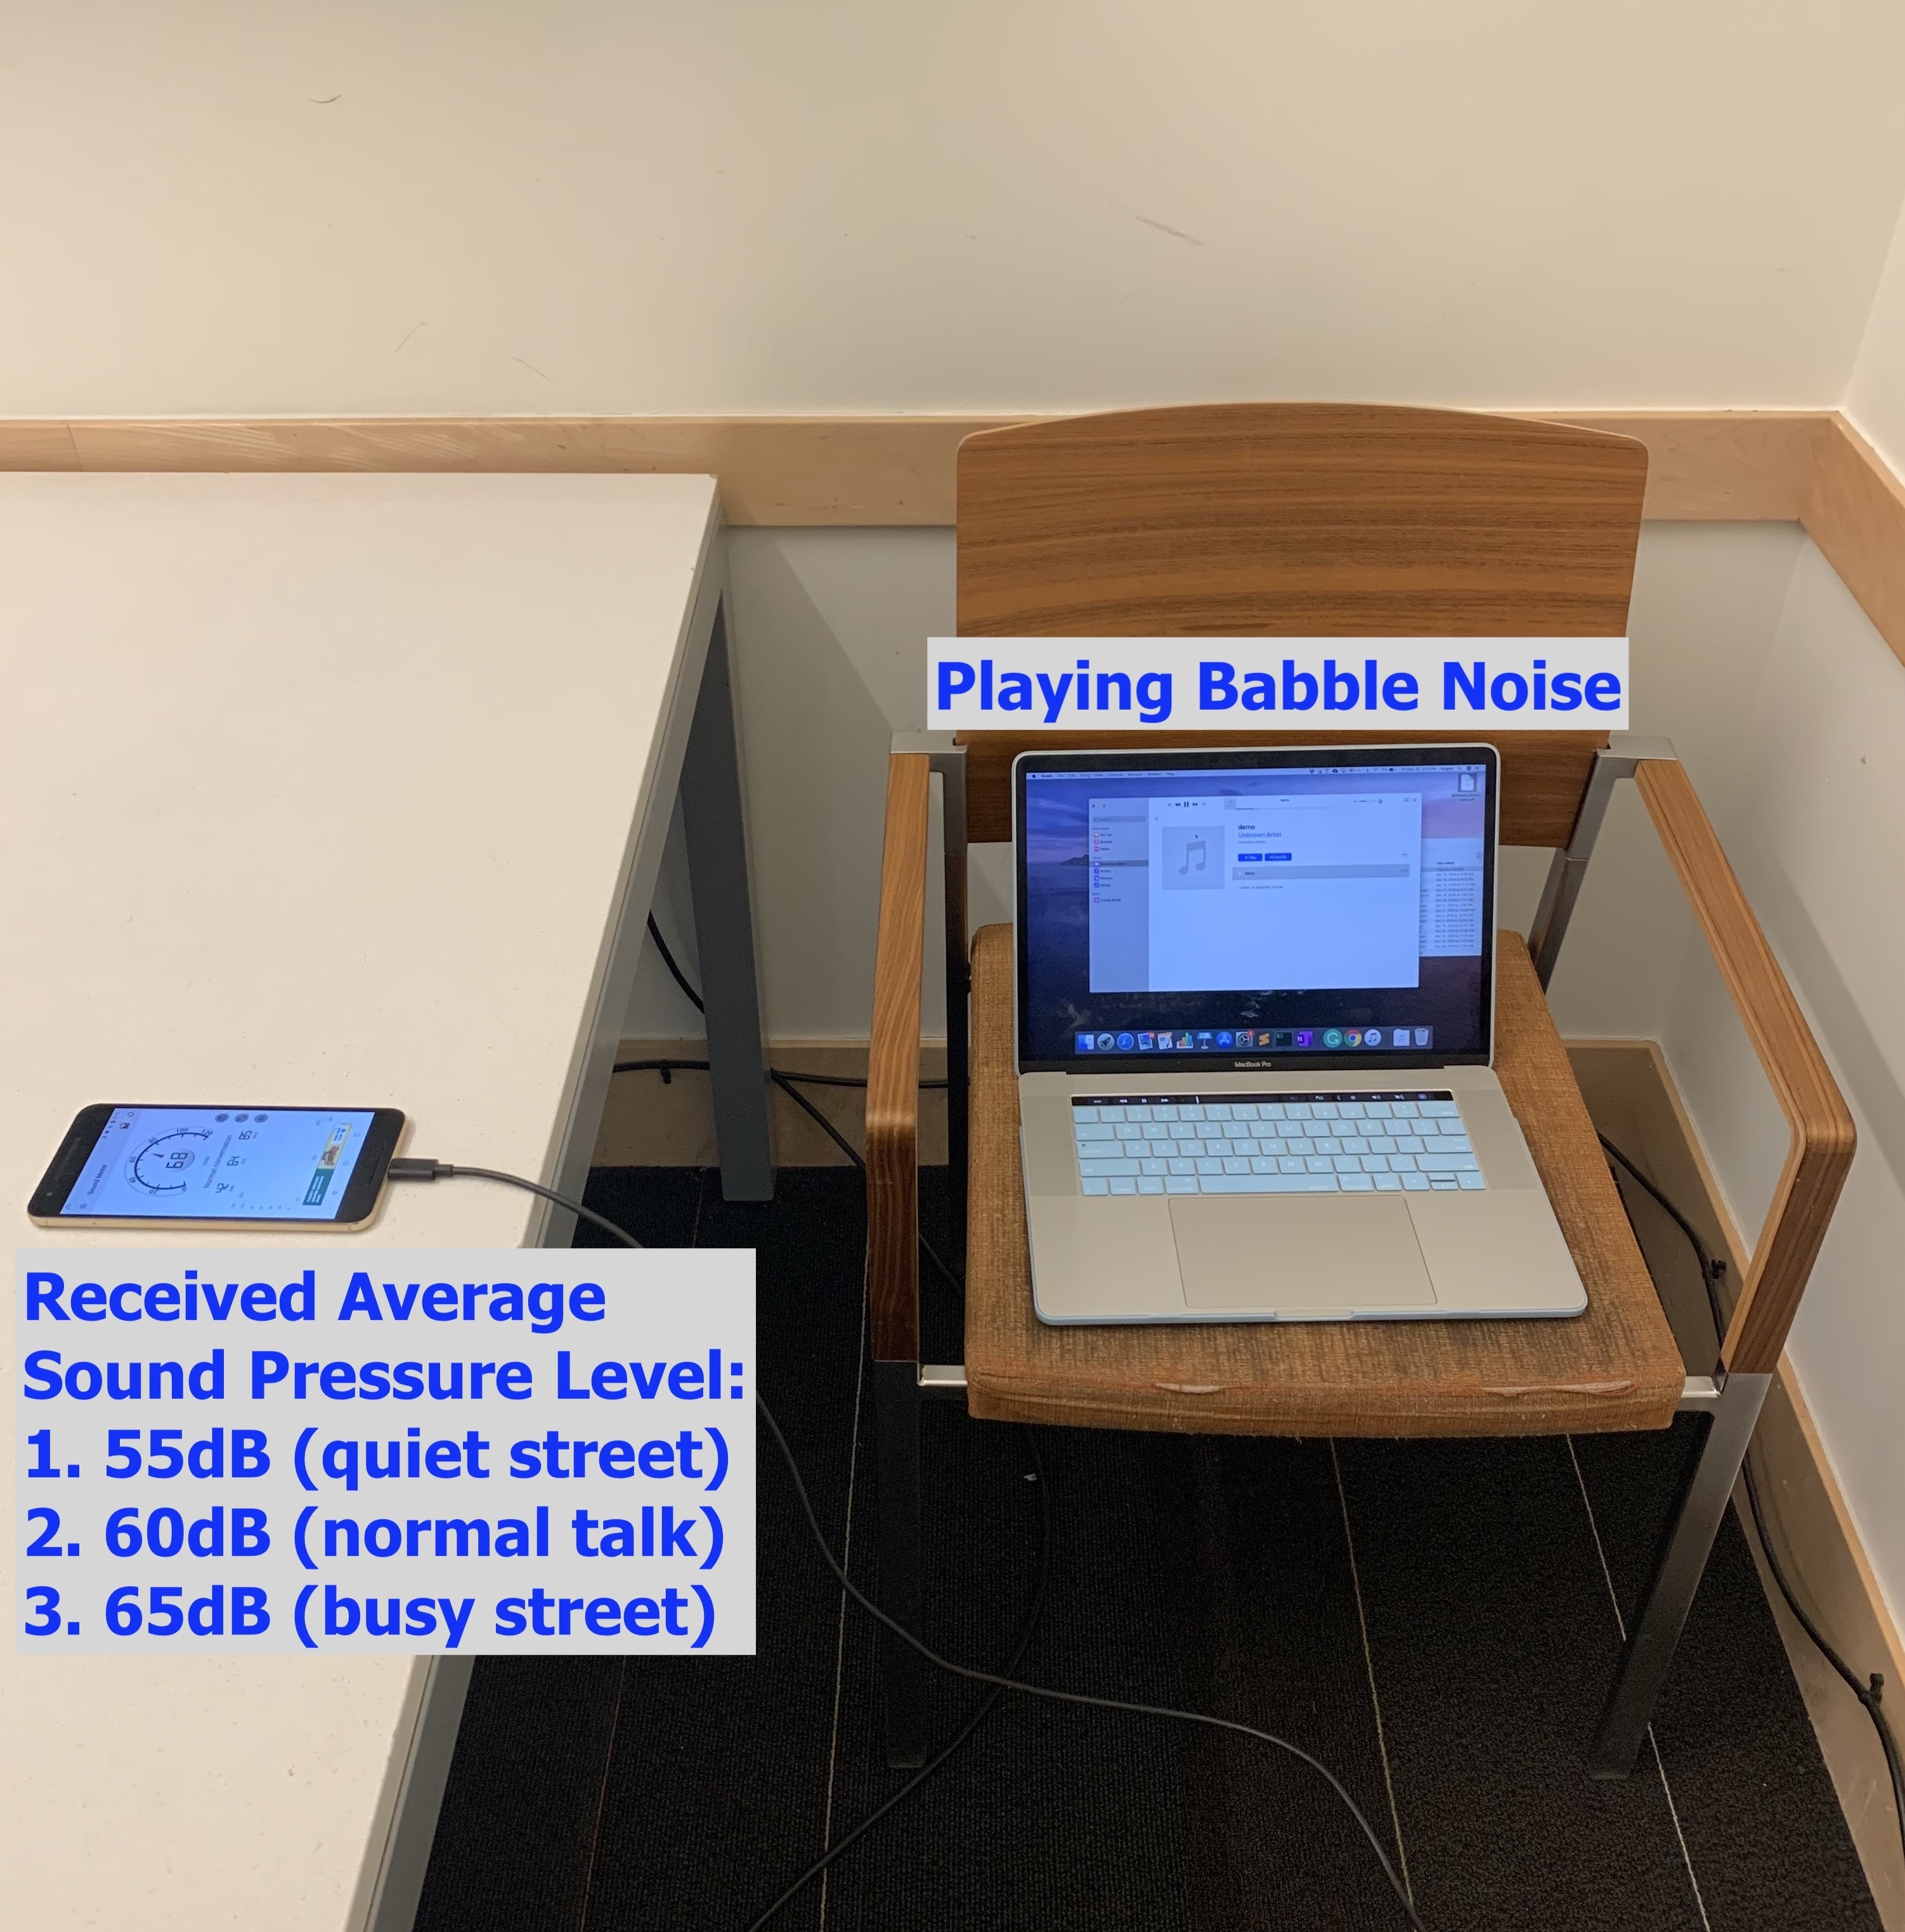
\includegraphics[width=.5\linewidth]{noisetest}
	\caption{Testing Setup.}
	\label{fig:noisetest}
\end{figure}

In this section, we test how background noises like real human talking influence the classification accuracy. When the smartphone speakers are playing sounds, a real person talks 20 cm away from the smartphone, with a similar volume. The result is shown in Figure~\ref{fig:noise}, the overall accuracy for all classes is about 60\%. Since {\systemName} still works in this experiment, it is an evidence that motion sensors are more sensitive to the built-in speakers than other sound sources that transmit signals through the air. 
%
It is worth mentioning that the performance of {\systemName} can be further improved if more training data is added. At this time, all training data are collected in a quiet environment, so directly feeding an input data from a noisy environment decreases the accuracy from 91\% to 60\%. Adding data from various environments, however, is expected to increase the robustness of the system and therefore a future research direction. 



To further test the impact of noises, we use a babble noise file and play the noise with different volumes. We control the sound pressure level received by the target phone to 55dB (quiet urban street), 60dB (normal conversation), and 65 dB (busy street). The results are shown in Figure ~\ref{fig:noisetestresult}.


\subsection{Impact of User Mobility}\label{sec:impact:move}
\begin{figure}[!h]
	\centering
	\includegraphics[width=.6\linewidth]{move}
	\caption{Impact of User Mobility.}
	\label{fig:move}
\end{figure}
All previous experiments are conducted when the smartphone is placed on a desk, without being touched or moved during the data collection stage. As illustrated in Figure~\ref{fig:spyphonepreprocess}, user movements are regarded as noises. Fortunately, since user movement is very slow and is unlikely to generate signals as high as 50 Hz. Thus, we can apply a high pass filter to mitigate the noise. In Figure~\ref{fig:newspec}, we see noises are removed after the filter. In this section, we validate the performance of {\systemName} with the presence of user mobility. 

We conduct two experiments: the walking scenario and the driving scenario. The users put the phone in their pockets while playing the sounds using the speakers. The results are shown in Figure~\ref{fig: walkanddrive}. The accuracy for the walking scenario is 83.94\% and that of driving scenario is 73.34\%. The accuracy of the driving scenario is relatively lower because of frequencies of the noises are relatively higher and thus close to the aliasing of human speech.



\begin{landscape}
	\begin{figure}[!h]
		
		\begin{minipage}[c]{.33\linewidth}
			\centering
			\includegraphics[width=\textwidth]{digitDB55CFM}
			\tiny
			\begin{tabular}{lr}
				\toprule
				Accuracy: 88.87\% & \hspace{-.00in} Error Rate: 11.13\% \\
				Precision: 88.87\% & \hspace{-.00in} True Positive Rate: 89.20\% \\
				$F_1$ Score: 0.889 & \hspace{-.00in} True Negative Rate: 98.89\% \\
				False Negative: 10.80\% & \hspace{-.00in} False Positive Rate: 1.11\% \\
				\bottomrule
			\end{tabular}
			\subcaption{Quiet Street (55 dB noise)}
		\end{minipage}
		\begin{minipage}[c]{.33\linewidth}
			\centering
			\includegraphics[width=\textwidth]{digitDB60CFM}
			\tiny
			\begin{tabular}{lr}
				\toprule
				Accuracy: 85.48\% & \hspace{-.00in} Error Rate: 14.52\% \\
				Precision: 85.49\% & \hspace{-.00in} True Positive Rate: 86.16\% \\
				$F_1$ Score: 0.855 & \hspace{-.00in} True Negative Rate: 98.55\% \\
				False Negative: 13.84\% & \hspace{-.00in} False Positive Rate: 1.45\% \\
				\bottomrule
			\end{tabular}
			\subcaption{Normal Conversation (60 dB noise)}
		\end{minipage}
		\begin{minipage}[c]{.33\linewidth}
			\centering
			\includegraphics[width=\textwidth]{digitDB65CFM}
			\tiny
			\begin{tabular}{lr}
				\toprule
				Accuracy: 77.50\% & \hspace{-.00in} Error Rate: 22.50\% \\
				Precision: 77.47\% & \hspace{-.00in} True Positive Rate: 77.61\% \\
				$F_1$ Score: 0.773 & \hspace{-.00in} True Negative Rate: 97.76\% \\
				False Negative: 22.39\% & \hspace{-.00in} False Positive Rate: 2.24\% \\
				\bottomrule
			\end{tabular}
		\subcaption{Noisy Street (65 dB noise)}
		\end{minipage}
		\caption[Impact of Surrounding Environments.]{The Impact of Surrounding Environments: Quiet Street, Normal Conversation, and Noisy Street. Note that the decibel values are the average sound pressure levels received by the smartphone. }
		\label{fig:noisetestresult}
	\end{figure}
\end{landscape}







\begin{landscape}
	\begin{figure}[!h]
		\centering
		\begin{minipage}[c]{.48\linewidth}
			\centering
			\includegraphics[width=\textwidth]{digitWalkCFM}
			\begin{tabular}{lr}
				\toprule
				Accuracy: 83.94\% & \hspace{-.00in} Error Rate: 16.06\% \\
				Precision: 83.94\% & \hspace{-.00in} True Positive Rate: 84.05\% \\
				$F_1$ Score: 0.839 & \hspace{-.00in} True Negative Rate: 98.39\% \\
				False Negative Rate: 15.95\% & \hspace{-.00in} False Positive Rate: 1.61\% \\
				\bottomrule
			\end{tabular}
		\end{minipage}
		\begin{minipage}[c]{.48\linewidth}
			\centering
			\includegraphics[width=\textwidth]{digitDriveCFM}
			\begin{tabular}{lr}
				\toprule
				Accuracy: 73.34\% & \hspace{-.00in} Error Rate: 26.66\% \\
				Precision: 73.34\% & \hspace{-.00in} True Positive Rate: 73.59\% \\
				$F_1$ Score: 0.733 & \hspace{-.00in} True Negative Rate: 97.34\% \\
				False Negative Rate: 26.41\% & \hspace{-.00in} False Positive Rate: 2.66\% \\
				\bottomrule
			\end{tabular}
		\end{minipage}
		\caption[Accuracy in the walking (left) and driving (right) scenario.]{Accuracy in the walking (left) and driving (right) scenario. The machine learning model trained in the stable environment is directly used to predict the testing data collected when user is walking or driving.}
		\label{fig: walkanddrive}
	\end{figure}
\end{landscape}



Moreover, we conduct an experiment in the extreme case that the user holds the phone in the hand and keeps moving it. The results are plotted in Figure~\ref{fig:move}, the average accuracy can still achieve 45\%.